% Reset-scoped official-render / Isaac-state evidence only.
\begin{figure}[t]
  \centering
  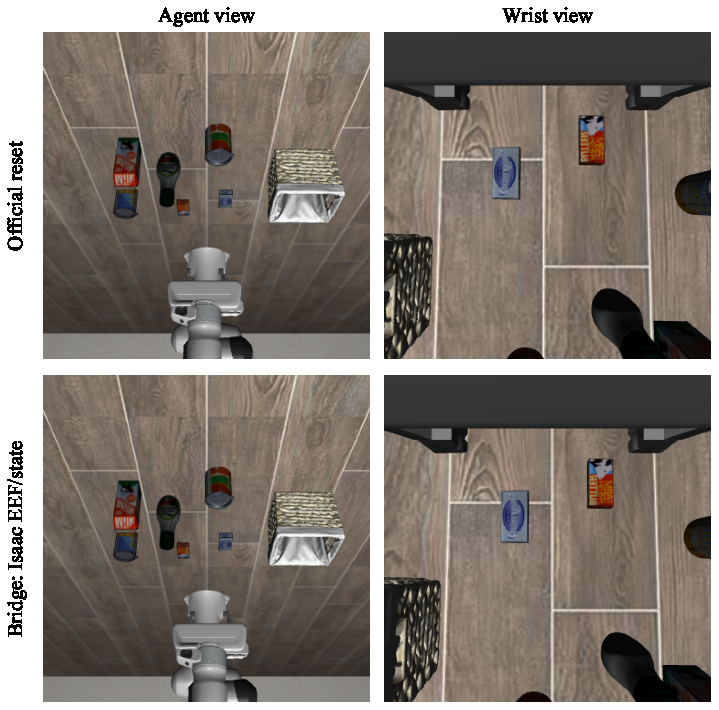
\includegraphics[width=0.76\textwidth]{outputs/xvla_isaac_official_render_bridge_v1_retry1/bridge_visual_comparison.pdf}
  \caption{Official-render observations for the same task, scene/object reset, and instruction. The top row is the official LIBERO reset; the bottom row retargets the canonical Panda end-effector pose and gripper from the measured Isaac reset. The robot state intentionally differs. This is a reset diagnostic, not task-success evidence.}
  \label{fig:xvla_bridge_visual}
\end{figure}

\begin{figure}[t]
  \centering
  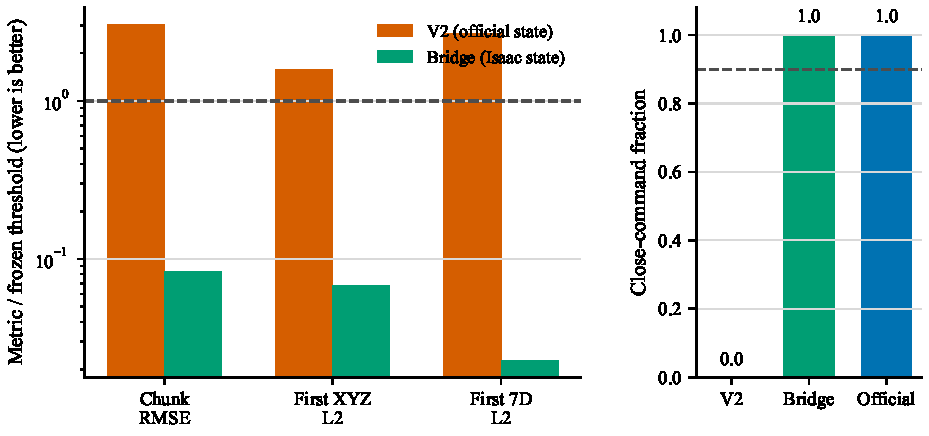
\includegraphics[width=0.82\textwidth]{outputs/xvla_isaac_official_render_bridge_v1_retry1/bridge_canary_gate_comparison.pdf}
  \caption{Unchanged frozen V2 thresholds applied over the same task, scene/object reset, instruction, and three paired seeds. In the left log-scale panel, each error metric is divided by its own threshold (dashed line at 1); bar heights show gate margin, not cross-metric effect size, and absolute values are in Table~\ref{tab:xvla_bridge_canary}. The right panel shows worst-seed close-command fraction (dashed gate at 0.9); Official is a reference bar. V2 uses native images with official state, while the bridge uses state-conditioned official-render images with mapped Isaac state. This is not a one-factor ablation or task-success evidence.}
  \label{fig:xvla_bridge_gate}
\end{figure}

\begin{figure}[t]
  \centering
  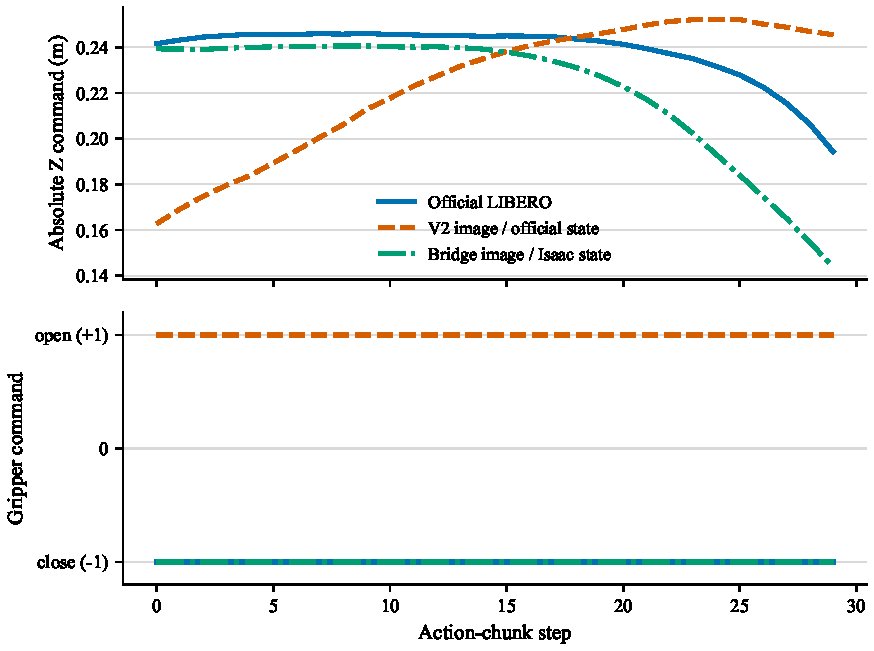
\includegraphics[width=0.72\textwidth]{outputs/xvla_isaac_official_render_bridge_v1_retry1/bridge_first_chunk_action_comparison.pdf}
  \caption{Mean predicted 30-step first action chunk after a single reset observation, over the same task, scene/object reset, instruction, and three paired inference seeds. V2 uses native images with official state; the state-conditioned official-render bridge uses mapped Isaac state. These are not executed closed-loop trajectories, a one-factor ablation, or task-success evidence.}
  \label{fig:xvla_bridge_actions}
\end{figure}
